%%%%%%%%%%%%%%%%%%%%%%%%
%%     Chapitre 1     %%
%%%%%%%%%%%%%%%%%%%%%%%%

\chapter{Chapitre 1} \label{chap1:titre}
\section{Section première}

\subsection{Sous-section}
Une référence dans le texte au diagramme de Feynman \ref{chap1:fig:feynman_0nu} ci-dessous.
\begin{figure}[ht!]
  \centering
  \scalebox{0.50}{\input{\chaponepdftextimgpath/Feynman_dbd_0nu.pdftex_t}}
  \caption{Exemple de figure .fig produite: Diagramme  de  Feynman de  la  \ddbsn{}  se produisant  par échange  d'un neutrino  de  Majorana massif  léger, interagissant  par courant gauche $V-A$.}
  \label{chap1:fig:feynman_0nu}
\end{figure}

\subsection{Sous-section}
Une référence dans le texte à l'image du spectre \ref{chap1:fig:dbd_spectre} ci-dessous.

\begin{figure}[ht!]
  \centering
  \scalebox{0.70}{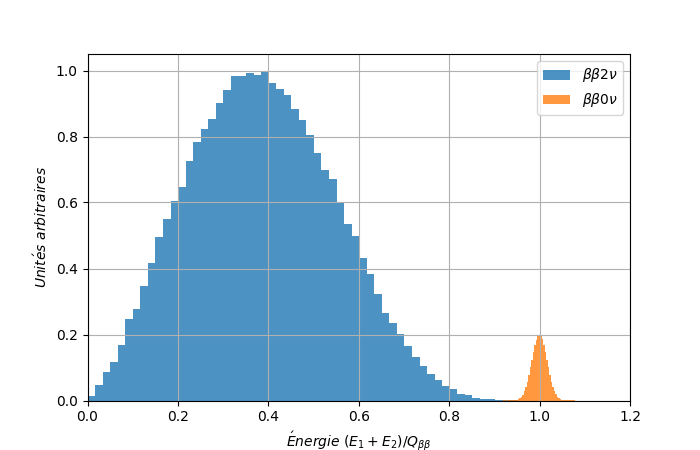
\includegraphics{\chaponeimgpath/dbd_spectre.png}}
  \caption{Exemple d'image png: Spectres  en énergie  \BBDN{}  (en bleu)  et \BBZN{}  (en orange) dégradés  par la résolution  en énergie expérimentale.   Un pic gaussien  est visible  à l'énergie  maximale \QBB{}  (les unités  sont
arbitraires).}
  \label{chap1:fig:dbd_spectre}
\end{figure}

\pagebreak
Un exemple de citation bibliographique: \cite{chap1_pauli_letter}.
